\begin{frame}
  \frametitle{Probabilistic Property Evaluation (PPE)}
  \begin{block}{Property Violation Probability}
    \begin{figure}
      \centering
      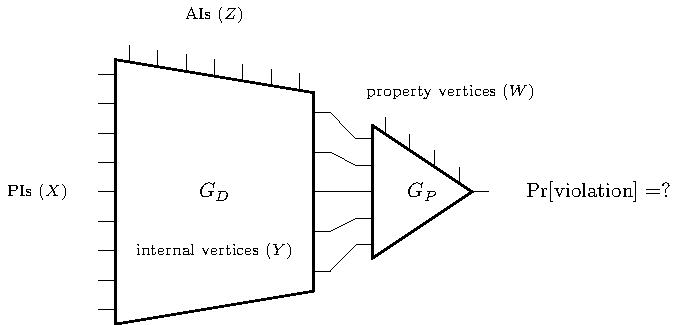
\includegraphics[scale=0.8]{fig/prob-spbn-miter.pdf}
    \end{figure}
    \pause
    \begin{itemize}
      \item PPE: the violation probability under $\pi:X\mapsto[0,1]$
            \pause
      \item MPPE: the maximum violation probability
    \end{itemize}
  \end{block}
\end{frame}

\begin{frame}
  \frametitle{Probabilistic Property Evaluation (PPE)}
  \begin{block}{Example: Probabilistic Equivalence Checking}
    \begin{figure}
      \centering
      \begin{circuitikz}[scale=0.4, transform shape]
    \tikzset{faulty/.style={muxdemux,muxdemux def={Lh=8,Rh=6,w=6,NL=7,NR=3,NB=0,NT=0},rotate=90}}
    \tikzset{golden/.style={muxdemux,muxdemux def={Lh=8,Rh=6,w=6,NL=4,NR=3,NB=0,NT=0},rotate=90}}
    \tikzset{black/.style={muxdemux,muxdemux def={Lh=1,Rh=0,w=1.5,NL=3,NR=1,NB=0,NT=0},rotate=90}}
    %\draw[step=1cm,gray,very thin] (-6,-6) grid (6,6); % For finding coordinates
    % Logic gates
    \node[faulty] (F) at (-2.5,-2) {};
    \node[golden] (G) at (2.5,-2) {};
    \node[xor port,rotate=90] (eq1) at (-2,1.7) {};
    \node[xor port,rotate=90] (eq2) at (0,1.7) {};
    \node[xor port,rotate=90] (eq3) at (2,1.7) {};
    \node[or port,rotate=90,number inputs=3] (and) at (0,3.5) {};
    \node[xor port,rotate=90,scale=0.5] (xor1) at (-3.5,-0.5) {};
    \node[black] (box1) at (-3.7,-2) {};
    \node[xor port,rotate=90,scale=0.5] (xor2) at (-1.5,-1) {};
    \node[black] (box2) at (-1.3,-2.5) {};
    % Wires
    \draw (F.rpin 1) -- (eq1.in 1);
    \draw (F.rpin 2) -- (eq2.in 1);
    \draw (F.rpin 3) -- (eq3.in 1);
    \draw (G.rpin 1) -- (eq1.in 2);
    \draw (G.rpin 2) -- (eq2.in 2);
    \draw (G.rpin 3) -- (eq3.in 2);
    \draw (eq1.out) -- (and.in 1);
    \draw (eq2.out) -- (and.in 2);
    \draw (eq3.out) -- (and.in 3);
    \draw (box1.rpin 1) -- ++(up:0.05cm) node{} -| (xor1.in 1);
    \draw (box2.rpin 1) -- ++(up:0.05cm) node{} -| (xor2.in 2);
    % Inputs
    \draw (F.lpin 1) -- ++(down:0.5cm) node{};
    \draw (F.lpin 2) -- ++(down:0.5cm) node{};
    \draw (F.lpin 3) -- ++(down:0.5cm) node{};
    \draw (G.lpin 1) -- ++(down:0.1cm) node[fill,circle,inner sep=1pt](c1){} -- ++(down:0.4cm){};
    \draw (c1) -| (F.lpin 4);
    \draw (G.lpin 2) -- ++(down:0.2cm) node[fill,circle,inner sep=1pt](c2){} -- ++(down:0.3cm){};
    \draw (c2) -| (F.lpin 5);
    \draw (G.lpin 3) -- ++(down:0.3cm) node[fill,circle,inner sep=1pt](c3){} -- ++(down:0.2cm){};
    \draw (c3) -| (F.lpin 6);
    \draw (G.lpin 4) -- ++(down:0.4cm) node[fill,circle,inner sep=1pt](c4){} -- ++(down:0.1cm){};
    \draw (c4) -| (F.lpin 7);
    % Labels
    \node at (-4,0) {$F$};
    \node at (4,0) {$G$};
    \node at (2.5,-5) {$X$};
    \node at (-3.75,-5) {$Z$};
    \node[font=\scriptsize] at (-3.25,-1.4) {$z_1$};
    \node[font=\scriptsize] at (-1.7,-1.9) {$z_2$};
\end{circuitikz}
    \end{figure}
    \pause
    \begin{itemize}
      \item PEC: the average difference probability under $\pi(x)=0.5$
            \pause
      \item MPEC: the maximum difference probability
    \end{itemize}
  \end{block}
\end{frame}